% Provenance (never printed): cycle 3 geography and "La planete Terre"
% (the great physical features of the world: relief, rivers, deserts, ice;
% reading a physical map); see sources/book1/PROVENANCE.md.
% Book 1, grade 4, chapter 3.
\chapter{世界自然地图}\label{ch:g4:world-physical-map}

萨米和诺尔在教室地板上展开一张大大的\omterm{def:g3:continents-and-oceans:world-map}{世界地图}，
他们跪在\omterm{def:g2:drawing-to-map:map}{地图}周围。这张\omterm{def:g2:drawing-to-map:map}{地图}和他们认识的\omterm{def:g2:drawing-to-map:map}{地图}不一样。
图上没有国家、边界和城镇。陆地用颜色来表示，
沿海和大片\omterm{def:g1:landscapes-around-us:landform}{平原}是绿色的，接着是浅黄色、棕色，
在少数地方则几乎是白色。\omterm{def:g2:water-on-earth:ocean}{海洋}也有几种蓝色：
靠近\omterm{def:g1:landscapes-around-us:water}{海岸}的颜色较浅，
离\omterm{def:g2:water-on-earth:ocean}{海洋}深处越远，颜色越深。

“亚洲那一块为什么是白色的？”诺尔问，“是雪吗？”不完全是。
在这张图上，每种颜色表示陆地有多高，或海水有多深。

\begin{recall}
\omterm{def:g2:drawing-to-map:map}{地图}从上方俯视、按比例缩小地呈现某个地方；\omterm{def:g2:drawing-to-map:legend}{图例}说明
它的颜色和符号（见\cref{ch:g2:drawing-to-map}）。陆地分为
七大洲，被五大洋环绕，\omterm{def:g3:continents-and-oceans:world-map}{世界地图}是展平的\omterm{def:g3:continents-and-oceans:globe}{地球仪}
（见\cref{ch:g3:continents-and-oceans}）。山、\omterm{def:g1:landscapes-around-us:landform}{丘陵}、\omterm{def:g1:landscapes-around-us:landform}{山谷}和\omterm{def:g1:landscapes-around-us:landform}{平原}
都是\omterm{def:g1:landscapes-around-us:landform}{地貌}；\omterm{def:g1:landscapes-around-us:water}{河流}从高处流向大海
（见\cref{ch:g1:landscapes-around-us}）。
\end{recall}

\section{读懂自然地图}

要说明某地有多高，需要一个全球通用的起点，
我们取\omterm{def:g4:world-physical-map:altitude}{海平面}作为起点。

\begin{definition}[海拔与海平面]\label{def:g4:world-physical-map:altitude}
\emph{海平面}\index{海平面}是海面的平均高度，
即涨潮与退潮之间的平均水位。某地的\emph{海拔}\index{海拔}
是该地高出海平面的高度，单位为米。海面以下则称
为\emph{深度}，即海底低于海平面的距离。
\end{definition}

海边城镇的\omterm{def:g4:world-physical-map:altitude}{海拔}只有几米。山区的村庄
可能位于 1\,500 米的高度：即高出\omterm{def:g4:world-physical-map:altitude}{海平面} 1.5 千米，
哪怕离任何\omterm{def:g1:landscapes-around-us:water}{海岸}有数百千米。

\begin{definition}[地形起伏]\label{def:g4:world-physical-map:relief}
某地区的\emph{地形起伏}\index{地形起伏}是指该地区陆地的形状：
哪里高、哪里低，以及\omterm{def:g4:world-physical-map:range}{山脉}、高原、\omterm{def:g1:landscapes-around-us:landform}{山谷}和
\omterm{def:g1:landscapes-around-us:landform}{平原}。
\end{definition}

\begin{definition}[自然地图]\label{def:g4:world-physical-map:physical-map}
\emph{自然地图}\index{自然地图}用颜色表示陆地的地形和海底的深度，
每种颜色对应一个\omterm{def:g4:world-physical-map:altitude}{海拔}或深度等级，
并标出大河、\omterm{def:g1:landscapes-around-us:water}{湖泊}、沙漠和冰原。
\end{definition}

\begin{omfigure}
\begin{tikzpicture}
\begin{axis}[ommap, width=\linewidth, xtick=\empty, ytick=\empty, grid=none,
    axis background/.style={}, clip=true]
  \addplot graphics[xmin=-180, xmax=180, ymin=-90, ymax=90]
    {figdata/out/grade-4-physical_map.png};
  \addplot[black!45, line width=0.15pt] table {figdata/out/shared-geo-land.dat};
  \addplot[fill=omHypsSeaB, draw=blue!60!black, line width=0.2pt]
    table {figdata/out/grade-4-physical_map-lakes.dat};
  \addplot[blue!70!black, line width=0.5pt] table {figdata/out/grade-4-physical_map-rivers.dat};
  \begin{scope}[every node/.style={font=\scriptsize\bfseries, align=center,
      fill=white, fill opacity=0.7, text opacity=1, inner sep=1pt, rounded corners=1pt}]
    \node at (axis cs:-112,47) {落基 \\山脉};
    \node at (axis cs:-62,-22) {安第斯山脉};
    \node at (axis cs:10,49) {阿尔卑斯山};
    \node at (axis cs:84,24) {喜马拉雅山};
    \node at (axis cs:4,23) {撒哈拉沙漠};
    \node at (axis cs:-40,74) {格陵兰 \\（冰）};
    \node at (axis cs:60,-80) {南极洲（冰）};
  \end{scope}
  \begin{scope}[every node/.style={font=\scriptsize\itshape, text=blue!50!black,
      fill=white, fill opacity=0.6, text opacity=1, inner sep=1pt}]
    \node at (axis cs:38,17) {尼罗河};
    \node at (axis cs:-56,-7) {亚马孙河};
    \node at (axis cs:-80,33) {密西西比河};
    \node at (axis cs:118,26) {长江};
  \end{scope}
\end{axis}
\end{tikzpicture}

\smallskip
\begin{tikzpicture}[font=\scriptsize, x=1.18cm]
  \foreach \i/\c/\t in {0/5A9CCF/{4000\\以下}, 1/84BCE0/{2000\\至 4000},
      2/B3D8EE/{200\\至 2000}, 3/DCEEF8/{0\\至 200}} {
    \definecolor{tmp}{HTML}{\c}
    \fill[tmp, draw=black!40] (\i,0) rectangle (\i+0.92,0.35);
    \node[align=center, anchor=north] at (\i+0.45,-0.05) {\t};
  }
  \foreach \i/\c/\t in {5/9CC98A/{0\\至 200}, 6/C9DE99/{200\\至 500},
      7/F1E7A8/{500\\至 1000}, 8/E5C58A/{1000\\至 2000}, 9/C79E76/{2000\\至 4000},
      10/ECE8E3/{4000\\以上}} {
    \definecolor{tmp}{HTML}{\c}
    \fill[tmp, draw=black!40] (\i,0) rectangle (\i+0.92,0.35);
    \node[align=center, anchor=north] at (\i+0.45,-0.05) {\t};
  }
  \node[anchor=south] at (2,0.4) {海水深度（m）};
  \node[anchor=south] at (8,0.4) {陆地海拔（m）};
\end{tikzpicture}

{\small 世界\omterm{def:g4:world-physical-map:physical-map}{自然地图}及其\omterm{def:g2:drawing-to-map:legend}{图例}。每种颜色表示一个
\omterm{def:g4:world-physical-map:altitude}{海拔}等级（陆地）或深度等级（海底）。\omterm{def:g1:landscapes-around-us:water}{河流}用深蓝色表示。
地形数据每隔一度纬度和经度取一个值绘制（约每 100 千米），
因此经过平滑处理，单个山峰和狭窄的海沟无法显示。
数据来源：NOAA ETOPO1 地形数据；\omterm{def:g1:landscapes-around-us:water}{河流}、\omterm{def:g1:landscapes-around-us:water}{湖泊}和
\omterm{def:g1:landscapes-around-us:water}{海岸}线取自 Natural Earth。}
\label{fig:g4:world-physical-map:map}
% ledger: data:etopo1, data:b1-ne-rivers, data:ne-land
\end{omfigure}

\begin{method}[读取自然地图上的颜色]\label{met:g4:world-physical-map:reading}
要查找\omterm{def:g4:world-physical-map:physical-map}{自然地图}上某地的\omterm{def:g4:world-physical-map:altitude}{海拔}：
\begin{enumerate}
  \item 找到该地点，并看它的颜色；
  \item 在\omterm{def:g2:drawing-to-map:legend}{图例}中找到相同的颜色；
  \item 读出它下方的色阶：该地点的\omterm{def:g4:world-physical-map:altitude}{海拔}介于
        两个数值之间。
\end{enumerate}
在海上求深度，方法相同。
\end{method}

\begin{example}[三处地点]\label{ex:g4:world-physical-map:three}
亚马孙河的河口位于南美洲\omterm{def:g1:landscapes-around-us:water}{海岸}，呈深绿色：其
\omterm{def:g4:world-physical-map:altitude}{海拔}介于 0 到 200 米之间。撒哈拉沙漠中部呈浅
绿色或淡黄色：\omterm{def:g4:world-physical-map:altitude}{海拔}介于 200 到 1\,000 米之间。喜马拉雅山以北的高原
位于亚洲，几乎呈白色：\omterm{def:g4:world-physical-map:altitude}{海拔}高于 4\,000 米。
\end{example}

\section{主要山脉}

在\omterm{def:g2:drawing-to-map:map}{地图}上，棕色和白色并非均匀分布。它们形成
狭长的条带。

\begin{definition}[山脉]\label{def:g4:world-physical-map:range}
称\emph{山脉}\index{山脉}为一长串相连的山，
连成一体、绵延数百至数千千米。
\end{definition}

安第斯\omterm{def:g4:world-physical-map:range}{山脉}纵贯南美洲西侧全境。北美洲
有落基\omterm{def:g4:world-physical-map:range}{山脉}，欧洲有阿尔卑斯山，亚洲则有
最高的\omterm{def:g4:world-physical-map:range}{山脉}——喜马拉雅山。那里矗立着地球上最高的山：珠穆朗玛峰，
高 8\,849 米，2020 年再次测量。
% ledger: tht:everest

\begin{omfigure}
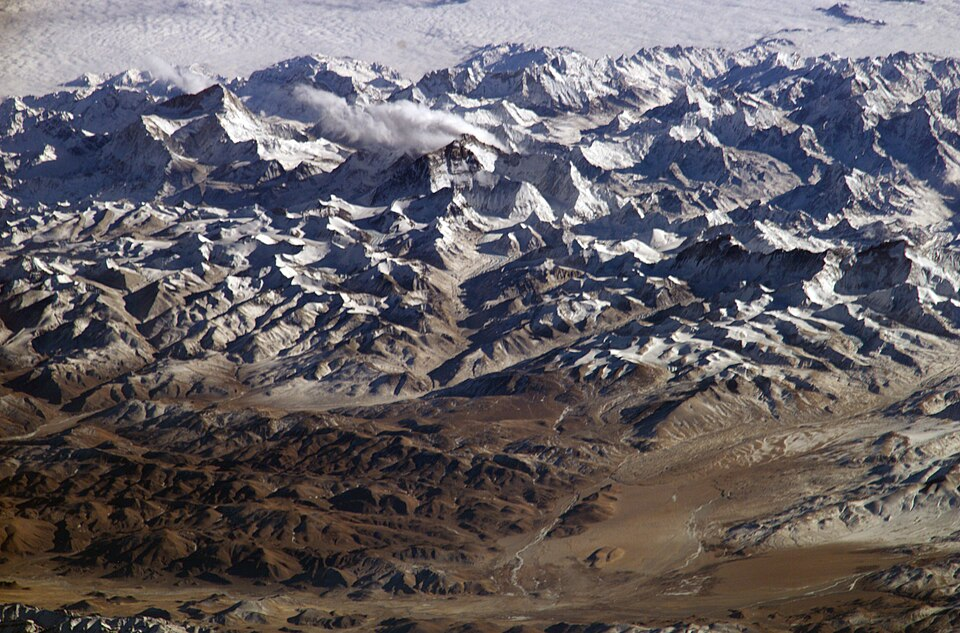
\includegraphics[width=0.75\linewidth]{images/book1/g4-himalaya-iss.jpg}

{\small 从国际空间站所见的喜马拉雅山，视线
朝南，自西藏高原望去：一片积雪覆盖的山峰宛如大海。
照片：NASA（公有领域）。}
% ledger: nasa:himalaya-iss
\end{omfigure}

\section{主要河流与湖泊}

雨水和融雪沿陆地流下，汇成溪流，再汇入
\omterm{def:g1:landscapes-around-us:water}{河流}，再由\omterm{def:g1:landscapes-around-us:water}{河流}把水带入大海。最大的\omterm{def:g1:landscapes-around-us:water}{河流}
汇集整个\omterm{def:g3:continents-and-oceans:continent}{大陆}地区的水。

地球上最长的两条\omterm{def:g1:landscapes-around-us:water}{河流}是非洲的尼罗河和
南美洲的亚马孙河。两者长度都接近 7\,000 千米。
哪一条最长？这并无定论，因为要看把起点定在哪里：
\omterm{def:g1:landscapes-around-us:water}{河流}从何处开始：在汇入它的所有小溪流中，
哪一条算作它真正的源头？2007 年，一支
沿亚马孙河追溯到更远源头的考察队称，其长约 6\,800 千米，
比尼罗河略长；许多参考书仍把尼罗河称为
最长的\omterm{def:g1:landscapes-around-us:water}{河流}。
% ledger: natgeo:nile, natgeo:amazon-nile-2007

毫无疑问，亚马孙河是最大的\omterm{def:g1:landscapes-around-us:water}{河流}：它的水量
超过其他任何\omterm{def:g1:landscapes-around-us:water}{河流}。
% ledger: natgeo:amazon-nile-2007

\begin{omfigure}
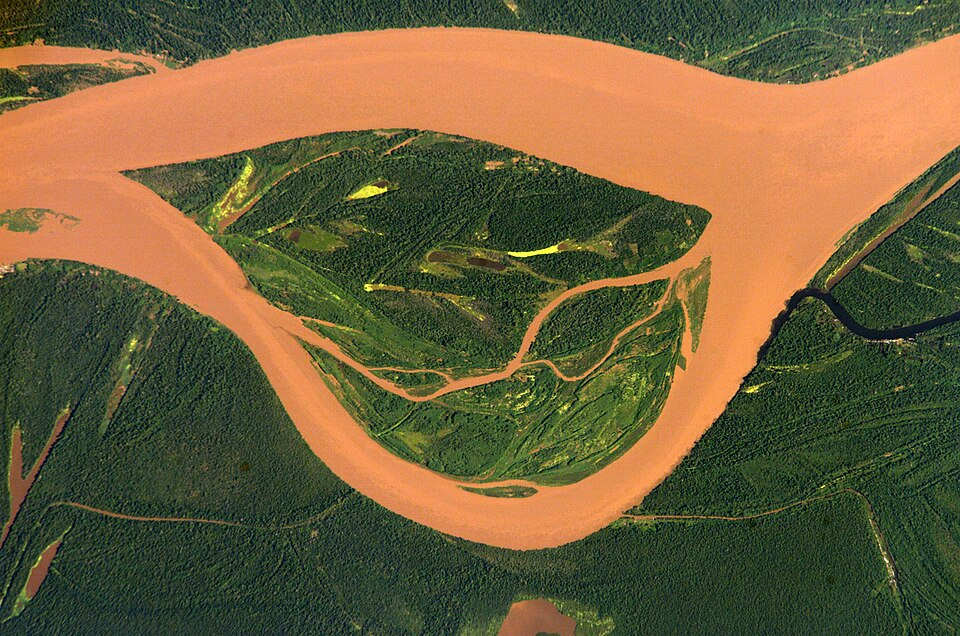
\includegraphics[width=0.6\linewidth]{images/book1/g4-amazon-iss.jpg}

{\small 亚马孙河被泥染成棕色，蜿蜒穿过雨林，
从国际空间站所见。照片：NASA（公有领域）。}
% ledger: nasa:amazon-iss
\end{omfigure}

\omterm{def:g1:landscapes-around-us:water}{湖泊}也屡创纪录。地球上最大的\omterm{def:g1:landscapes-around-us:water}{湖泊}是里海，
位于欧洲和亚洲之间：它大到被称为海，但它
四周都被陆地环绕。它的面积超过
370\,000 平方千米。最深的\omterm{def:g1:landscapes-around-us:water}{湖泊}是俄罗斯的贝加尔湖：在
某些地方，湖底低于水面近 2 千米。
% ledger: natgeo:caspian-baikal

\section{沙漠与大冰原}

\omterm{def:g4:world-physical-map:physical-map}{自然地图}上有两类地方格外醒目，因为那里几乎
没有植物生长：广袤的沙漠，那里几乎从不下雨，以及大
冰原。

撒哈拉沙漠位于非洲北部，是地球上最大的热沙漠。它
面积约八百五十万平方千米。非洲全境
面积约 3000 万平方千米，因此撒哈拉沙漠略多于
非洲面积的四分之一：超过 $\frac{1}{4}$，但小于
$\frac{1}{3}$。
% ledger: natgeo:sahara, data:etopo1

大冰原覆盖\omterm{def:g3:continents-and-oceans:poles}{南极}洲，环绕\omterm{def:g3:continents-and-oceans:poles}{南极}，并覆盖
格陵兰岛的大部分，位于大西洋最北端。那里的雪经过数千
年积累，形成厚厚的冰层。在\omterm{def:g4:world-physical-map:physical-map}{自然地图}上，它们的颜色与高地相同，
因为冰顶远高于\omterm{def:g4:world-physical-map:altitude}{海平面}。

\section{最高与最深}

\omterm{def:g4:world-physical-map:physical-map}{自然地图}显示了地表的形态，但它
太小，掩盖了这些极端情况。下面按比例将它们并排比较。

\begin{omfigure}
\begin{tikzpicture}[x=1cm, y=0.32cm, font=\small]
  % sea level
  \fill[omHypsSeaA] (0,0) rectangle (9,-11.5);
  \fill[omHypsSeaD!80] (4.6,-11.5) -- (4.6,-11.0) -- (5.0,-10.98) -- (5.4,-11.0) -- (5.4,-11.5) -- cycle;
  \draw[black!60] (-0.2,0) -- (9.2,0);
  \node[anchor=west, font=\scriptsize] at (9.25,0) {海平面，0\,m};
  % height scale
  \draw[black!60] (0,-11.5) -- (0,10);
  \foreach \h in {-10,-8,...,8} {
    \draw[black!60] (-0.1,\h) -- (0,\h);
    \node[anchor=east, font=\scriptsize] at (-0.12,\h) {\h\,km};
  }
  % ocean floor and trench
  \fill[brown!45] (0.05,-11.5) -- (0.05,-3.7) -- (3.2,-3.7) -- (4.4,-6) -- (4.9,-10.98) -- (5.1,-10.98)
    -- (5.6,-6) -- (6.4,-3.7) -- (9,-3.7) -- (9,-11.5) -- cycle;
  \node[font=\scriptsize, align=center] at (2.0,-5.3) {洋底，\\深约 3\,700\,m};
  \node[font=\scriptsize, anchor=west, align=left] at (5.6,-9.4) {最深点：\\挑战者深渊，\\接近 11\,000\,m};
  % Everest
  \fill[black!35] (6.6,0) -- (7.6,8.85) -- (8.6,0) -- cycle;
  \fill[white, draw=black!45, line width=0.3pt] (7.35,6.6) -- (7.6,8.85) -- (7.85,6.6) -- (7.6,7.1) -- cycle;
  \node[font=\scriptsize, align=center, anchor=south] at (7.6,8.95) {珠穆朗玛峰，8\,849\,m};
  % cirrus clouds band
  \draw[black!45, line width=0.6pt] (1.0,9.0) .. controls (1.6,9.5) and (2.2,9.1) .. (2.8,9.6);
  \draw[black!45, line width=0.6pt] (1.2,8.3) .. controls (1.8,8.8) and (2.4,8.4) .. (3.0,8.9);
  \node[font=\scriptsize, align=center] at (2.0,7.2) {高云 \\（卷云）};
  % a village
  \fill[black!60] (2.2,1.5) rectangle (2.45,1.75);
  \node[font=\scriptsize, anchor=west] at (2.5,1.6) {山村，1\,500\,m};
\end{tikzpicture}

{\small 从\omterm{def:g2:water-on-earth:ocean}{海洋}最深处到最高峰，按
比例绘制。挑战者深渊位于太平洋，其海面以下的深度
超过珠穆朗玛峰高出海面的高度。数值：珠穆朗玛峰 8\,849\,m；
挑战者深渊近 11\,000\,m；\omterm{def:g2:water-on-earth:ocean}{海洋}平均海底约
3\,700\,m。}
\label{fig:g4:world-physical-map:extremes}
% ledger: tht:everest, usgs:trench-depth, nos:ocean-depth, wmo:cloud-levels
\end{omfigure}

\begin{example}[深渊中的珠穆朗玛峰]\label{ex:g4:world-physical-map:everest-in-deep}
设想把珠穆朗玛峰搬起来，放到
挑战者深渊的底部，其峰顶仍会在水下：海沟约深 11\,000
米，而山峰高 8\,849 米。其峰顶仍被超过 2
千米的海水覆盖。
% ledger: tht:everest, usgs:trench-depth
\end{example}

\section{练习}

\begin{exercise}[$\star$]\label{exo:g4:world-physical-map:1}
某地的\omterm{def:g4:world-physical-map:altitude}{海拔}是什么？它是从哪个水平面起算的？
\end{exercise}

\begin{exercise}[$\star$]\label{exo:g4:world-physical-map:2}
利用\omterm{def:g4:world-physical-map:physical-map}{自然地图}的\omterm{def:g2:drawing-to-map:legend}{图例}，给出一处
颜色为 (a) 深绿色；(b) 淡黄色；(c) 近白色的地方的\omterm{def:g4:world-physical-map:altitude}{海拔}。
\end{exercise}

\begin{exercise}[$\star$]\label{exo:g4:world-physical-map:3}
求下列各处分别位于哪个\omterm{def:g3:continents-and-oceans:continent}{大陆}：(a) 安第斯\omterm{def:g4:world-physical-map:range}{山脉}；(b) 喜马拉雅\omterm{def:g4:world-physical-map:range}{山脉}；(c) 撒哈拉沙漠；
(d) 落基\omterm{def:g4:world-physical-map:range}{山脉}？
\end{exercise}

\begin{exercise}[$\star$]\label{exo:g4:world-physical-map:4}
写出地球上最高的山、最大的湖和最深的湖。
\end{exercise}

\begin{exercise}[$\star$]\label{exo:g4:world-physical-map:5}
在\omterm{def:g4:world-physical-map:physical-map}{自然地图}上，靠近\omterm{def:g1:landscapes-around-us:water}{海岸}的海域呈浅蓝色，大洋中部
呈深蓝色。这说明了海的深度有什么特点？
\end{exercise}

\begin{exercise}[$\star$]\label{exo:g4:world-physical-map:6}
为什么\omterm{def:g3:continents-and-oceans:poles}{南极}洲和格陵兰岛在\omterm{def:g4:world-physical-map:physical-map}{自然地图}上
的颜色与高地相同？
\end{exercise}

\begin{exercise}[$\star\star$]\label{exo:g4:world-physical-map:7}
按从低到高的顺序排列：海滩；位于
1\,500 米的山村；珠穆朗玛峰峰顶；挑战者
深渊底部；\omterm{def:g2:water-on-earth:ocean}{海洋}的平均海底。
\end{exercise}

\begin{exercise}[$\star\star$]\label{exo:g4:world-physical-map:8}
为什么我们无法确定尼罗河和亚马孙河
哪条是最长的\omterm{def:g1:landscapes-around-us:water}{河流}？
\end{exercise}

\begin{exercise}[$\star\star$]\label{exo:g4:world-physical-map:9}
非洲面积约 3000 万平方千米。其中哪部分是
四分之一？三分之一？撒哈拉沙漠面积约八百五十万
平方千米：它比非洲面积的四分之一多还是少？比
三分之一多还是少？
\end{exercise}

\begin{exercise}[$\star\star$]\label{exo:g4:world-physical-map:10}
一座山地小屋\omterm{def:g4:world-physical-map:altitude}{海拔} 2\,500 米，其下方一座\omterm{def:g1:landscapes-around-us:water}{湖泊}\omterm{def:g4:world-physical-map:altitude}{海拔} 1\,000
米。小屋比\omterm{def:g1:landscapes-around-us:water}{湖泊}高多少米？它们在\omterm{def:g4:world-physical-map:physical-map}{自然地图}上
各是什么颜色？
\end{exercise}

\begin{exercise}[$\star\star\star$]\label{exo:g4:world-physical-map:11}
一架飞机在\omterm{def:g4:world-physical-map:altitude}{海平面}以上 10 千米处飞行。它是否比珠穆朗玛峰
更高？高出多少米？若它飞过挑战者深渊，
它离海沟底部有多高（取 11\,000 米
为海沟深度）？
\end{exercise}
